\chapter{基于多视图特征的移动应用识别方法}\label{chap:AIBMF}
对于HTTPS加密流量,传统的DPI方法已经不能够有效地完成识别任务,而基于经典机器学习算法的识别方法需要依赖特征工程手段进行特征设计,并且这些特征很容易受到网络环境的影响而不具备鲁棒性。因此,本章将从多个视图角度对HTTPS流量进行特征建模形成多视图特征,并在此基础上使用深度学习模型进行高阶特征学习和融合,最后完成移动应用识别任务。

\section{引言}
基于HTTPS流量的移动应用识别是指对被动观察的HTTPS加密网络数据流与产生其的具体移动应用进行关联映射的过程。本文的研究工作是建立在对HTTPS流量以下三个方面的认知:

\emph{(i)} SSL/TLS协议本质上是移动应用客户端和服务器之间通信的一种语言,这种语言的具体表现是数据包序列;

\emph{(ii)}因为协议状态机是对网络流的总体抽象描述,所以可以从不同的协议状态信息中构造应用指纹。如消息类型,内容类型等协议定义的参数信息。

\emph {(iii)}尽管SSL/TLS隐藏了网络流的有效负载,但仍然从加密连接中泄漏可以用于流量识别的状态信息。

基于以上,采取深度学习的方法,从不同的视图特征进行研究,使用深度学习的方法提取抽象的特征,构建识别的模型。



\section{方法阐述}
本章提出了一种基于多视图特征的移动应用识别方法---\emph{AIBMF}\footnote{Mobile \underline{A}pplication \underline{I}dentification Over HTTPS Traffic \underline{B}ased on \underline{M}ulti-view \underline{F}eatures},该方法的架构如图\ref{fig:AIBMF-Architecture}所示,由预处理、特征学习、流量识别三个阶段构成。在预处理时,对原始的数据流样本从多个角度抽取特征,形成多视图特征;在特征学习时,对多视图特征采用深度学习模型方法学习高阶抽象特征;在应用识别时,进行特征融合并使用全连接神经网络完成分类任务。
\begin{figure}[!htbp]
	\centering
	\includegraphics[width=0.80\textwidth]{AIBMF-model.pdf}
	\bicaption{AIBMF网络结构。}{AIBMF Architecture.}
	\label{fig:AIBMF-Architecture}
\end{figure}

\subsection{数据流预处理}
在第三章将流量数据按照流进行提取,形成的数据集中每一条流就是一个待识别的样本。整个流的集合可以表示为:
\begin{equation}
    D = \{{\{f_i\}}_{i=1}^{i=N}\}_{j=1}^{j=C} 
\end{equation}
这里$f_i$表示第$i$条流,$N$表示当前应用的样本数目,$C$表示的是应用的个数。从流量数据包的负载、内容类型以及大小三个视图角度提取初始特征,具体阐述如下。

\subsubsection{负载视图}
如图\ref{fig:wireshark-payload}所示,负载部分由ASCII码构成。
\begin{figure}[!htbp]
	\centering
	\includegraphics[width=0.35\textwidth]{Wireshark-payload.png}
	\bicaption{流量负载。}{Payload.}
	\label{fig:wireshark-payload}
\end{figure}
如下是数据集中前20款应用在负载的ASCII编码的分布情况。对于单个应用,将其所有流的所有包的负载按照字节的ASCII编码转换为0-255的数值,统计所有取值的数量,绘制箱式图。如图\ref{fig:payload-eda}所示,图中方块的上边界表示的是上四分位数,中间红色菱形块表示的是平均数,中间黄色实线表示的是中位数。可以发现针对不同的应用,负载的ASCII码在上四分位数、中位数、平均数上的取值均存在差异,为了更加进一步探索负载对于流量识别的作用,本文将其定义为负载视图。
\begin{figure}[!htbp]
	\centering
	\includegraphics[width=0.80\textwidth]{payload-eda.png}
	\bicaption{流量负载字节分布。}{Payload distribution.}
	\label{fig:payload-eda}
\end{figure}
%-------------------------------------------------------------------------
\subsubsection{内容类型视图}
内容类型(content type)是SSL/TLS协议定义的,取值范围及其意义见表\ref{tab:content-type}, 在HTTPS的通信过程中,其对于流中每一个数据包进行了标记。
\begin{table}[!htbp]
    \bicaption{内容类型。}{Content Type.}
    \label{tab:content-type}
    \centering
    \footnotesize% fontsize
    \setlength{\tabcolsep}{4pt}% column separation
    \renewcommand{\arraystretch}{1.2}%row space
    \resizebox{\columnwidth}{!}{
        \begin{tabular}{rccc}
        \textbf{取值} & \textbf{描述} & \textbf{DTLS-OJ} & \textbf{参考}\\
        \hline
        0-19 & Unassigned (Requires coordination; see [RFC7983]) & & [RFC5764][RFC7983]\\
        20 & change\_cipher\_spec & Y & [RFC8446]\\
        21 & alert & Y & [RFC8446]\\
        22 & handshake & Y & [RFC8446]\\
        23 & application\_data & Y & [RFC8446]\\
        24 & heartbeat & Y & [RFC6520]\\
        25 & tls12\_cid (TEMPORARY - registered 2019-07-02, expires 2020-07-02) & Y & [draft-ietf-tls-dtls-connection-id]\\
        26-63 & Unassigned & & \\
        64-255 & Unassigned (Requires coordination; see [RFC7983]) & & [RFC5764][RFC7983]\\
        \hline
        \end{tabular}    
    }

\end{table}
接着比较了数据集中前20款应用在内容类型(content type)的取值的分布情况。图\ref{fig:content-type-eda}是四种应用的箱式图,可以发现这四款应用的内容类型的取值在上四分位数、中位数、平均数上存在显著的差异。为了更加进一步探索content type对于流量识别的作用,本文将其定义为内容类型视图。
\begin{figure}[!htbp]
	\centering
	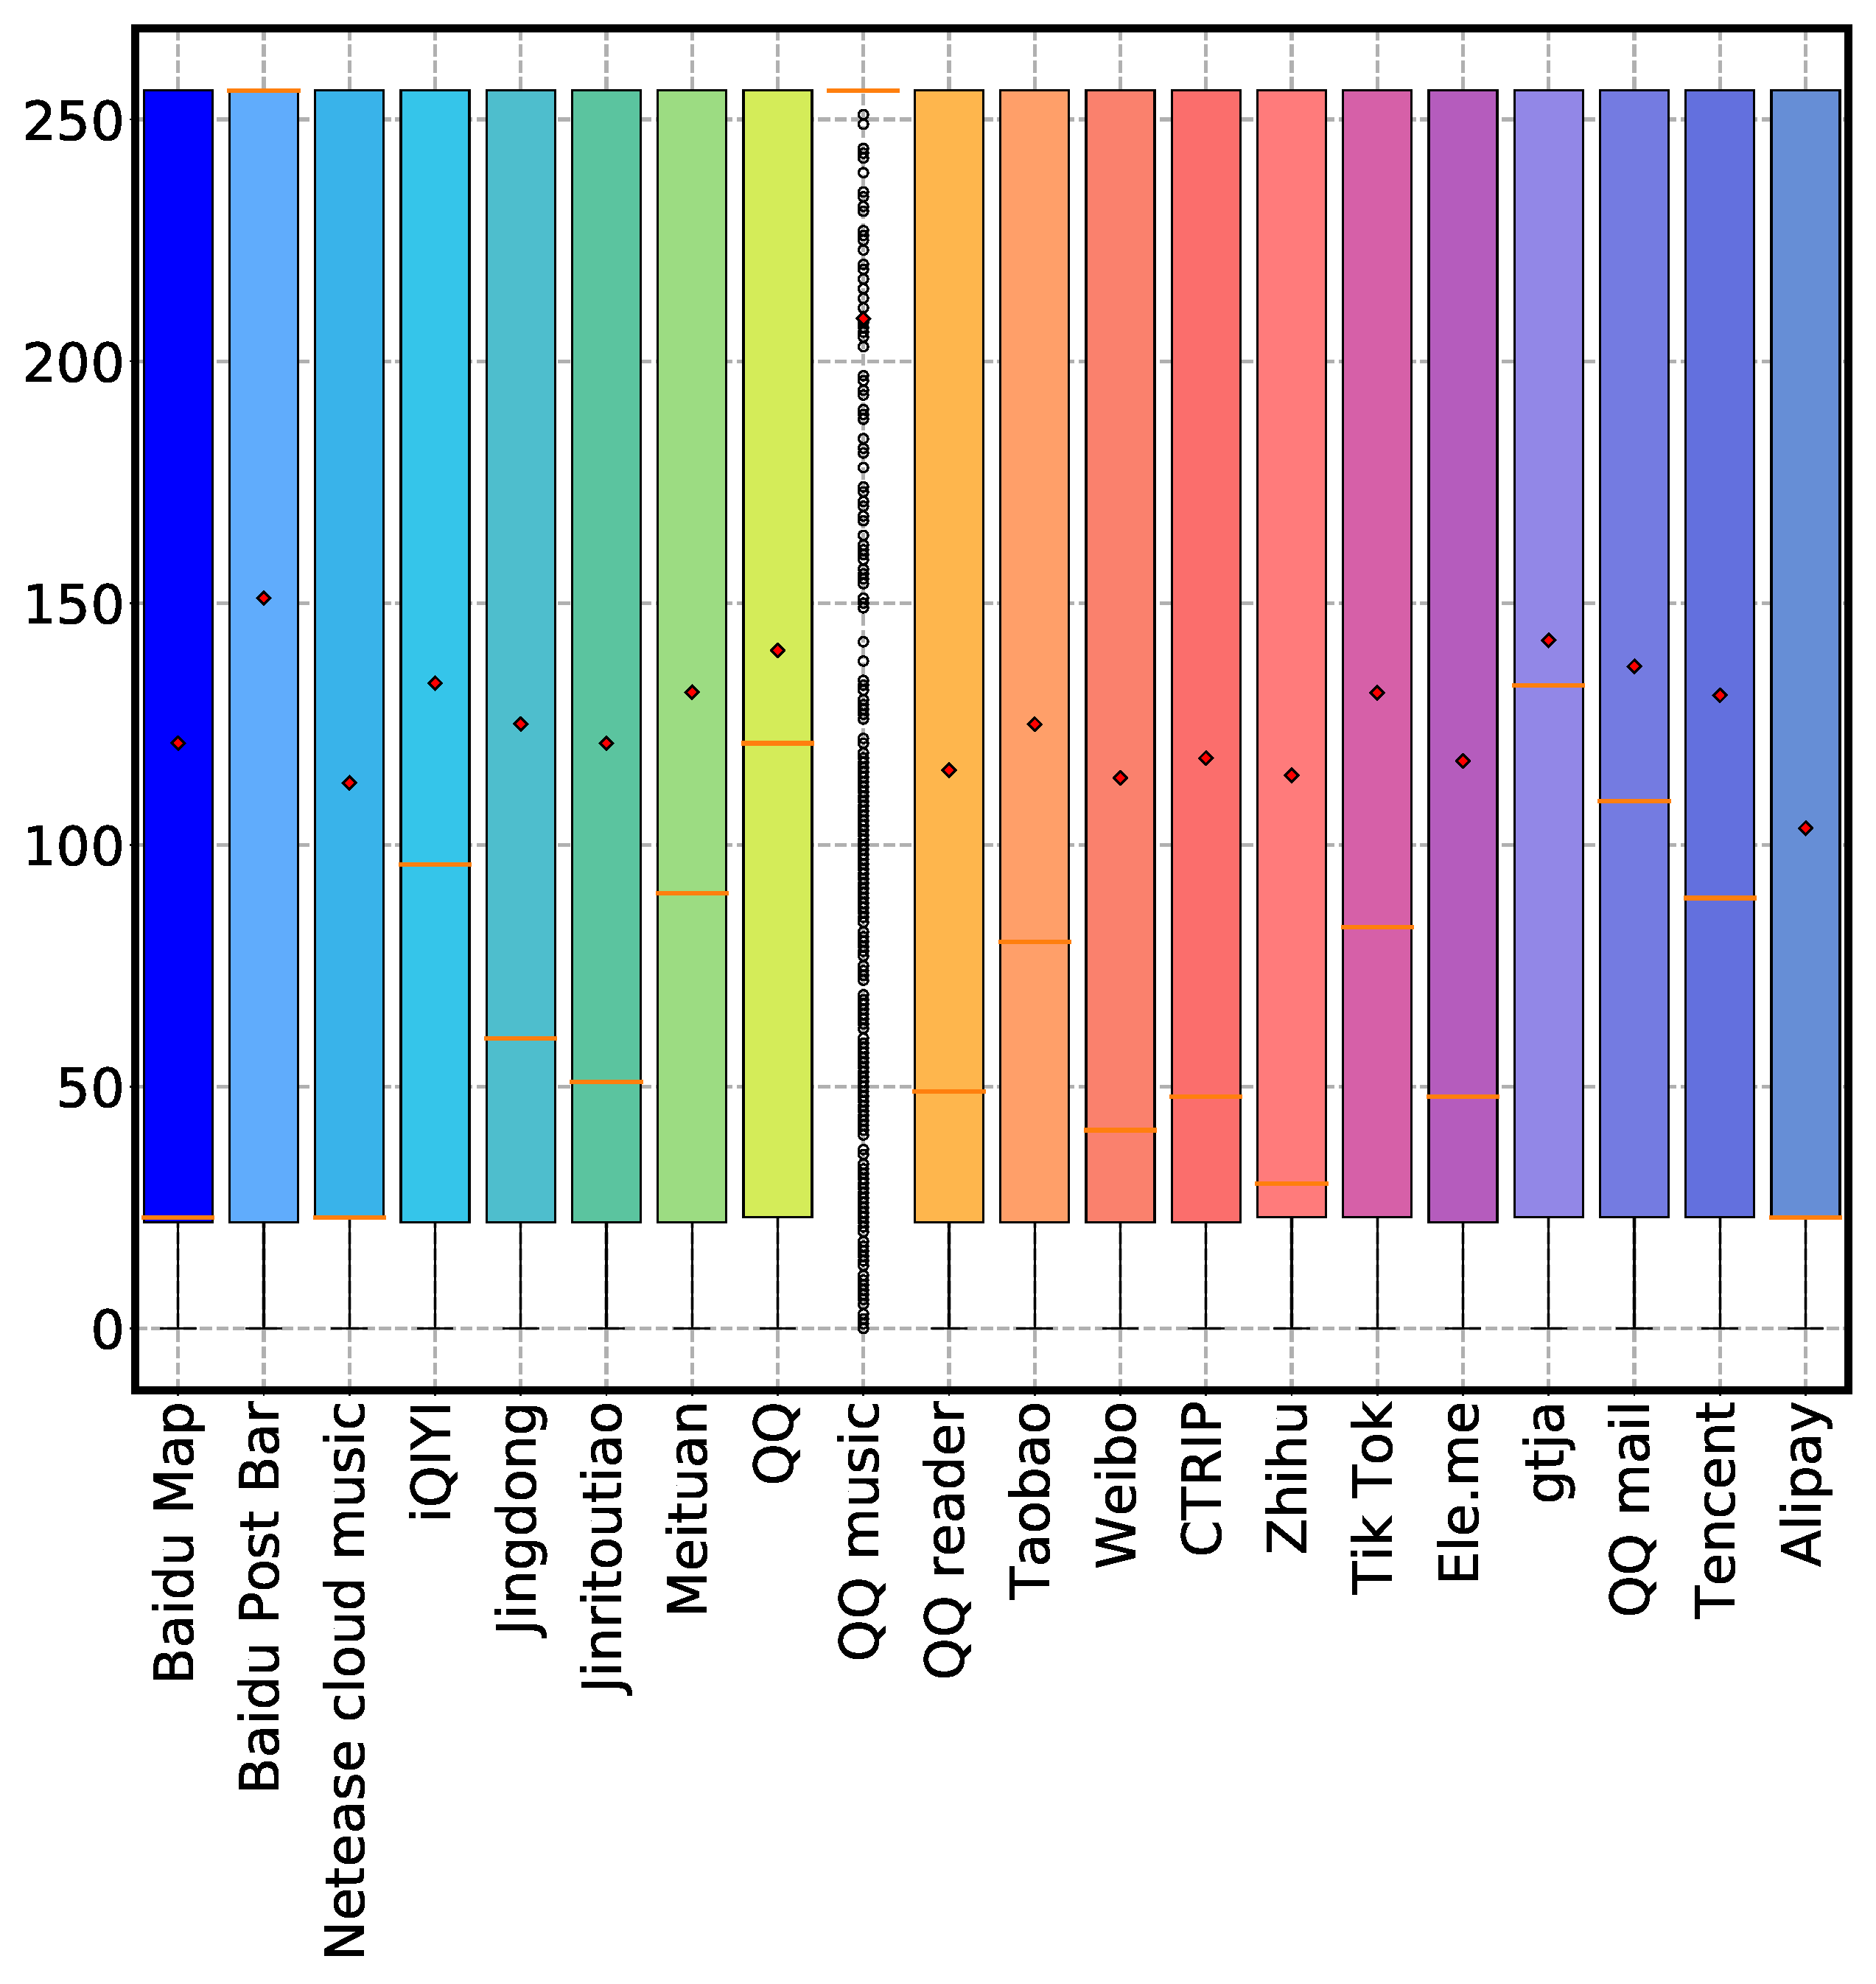
\includegraphics[width=0.80\textwidth]{content-type-eda.eps}
	\bicaption{内容类型分布。}{Content type distribution.}
	\label{fig:content-type-eda}
\end{figure}




%-----------------------------------------------------------------------
\subsubsection{数据包大小视图}
最后比较了数据集中前20款应用在数据包大小的分布情况。对于单个应用的所有样本流的所有数据包的大小进行统计。如图\ref{fig:packet-size-eda}所示,不同的应用的数据包在大小在上四分位数、中位数、平均数上存在显著的差异,为了更加进一步探索数据包大小对于流量识别的作用,本文将其定义为数据包大小视图。
\begin{figure}[!htbp]
	\centering
	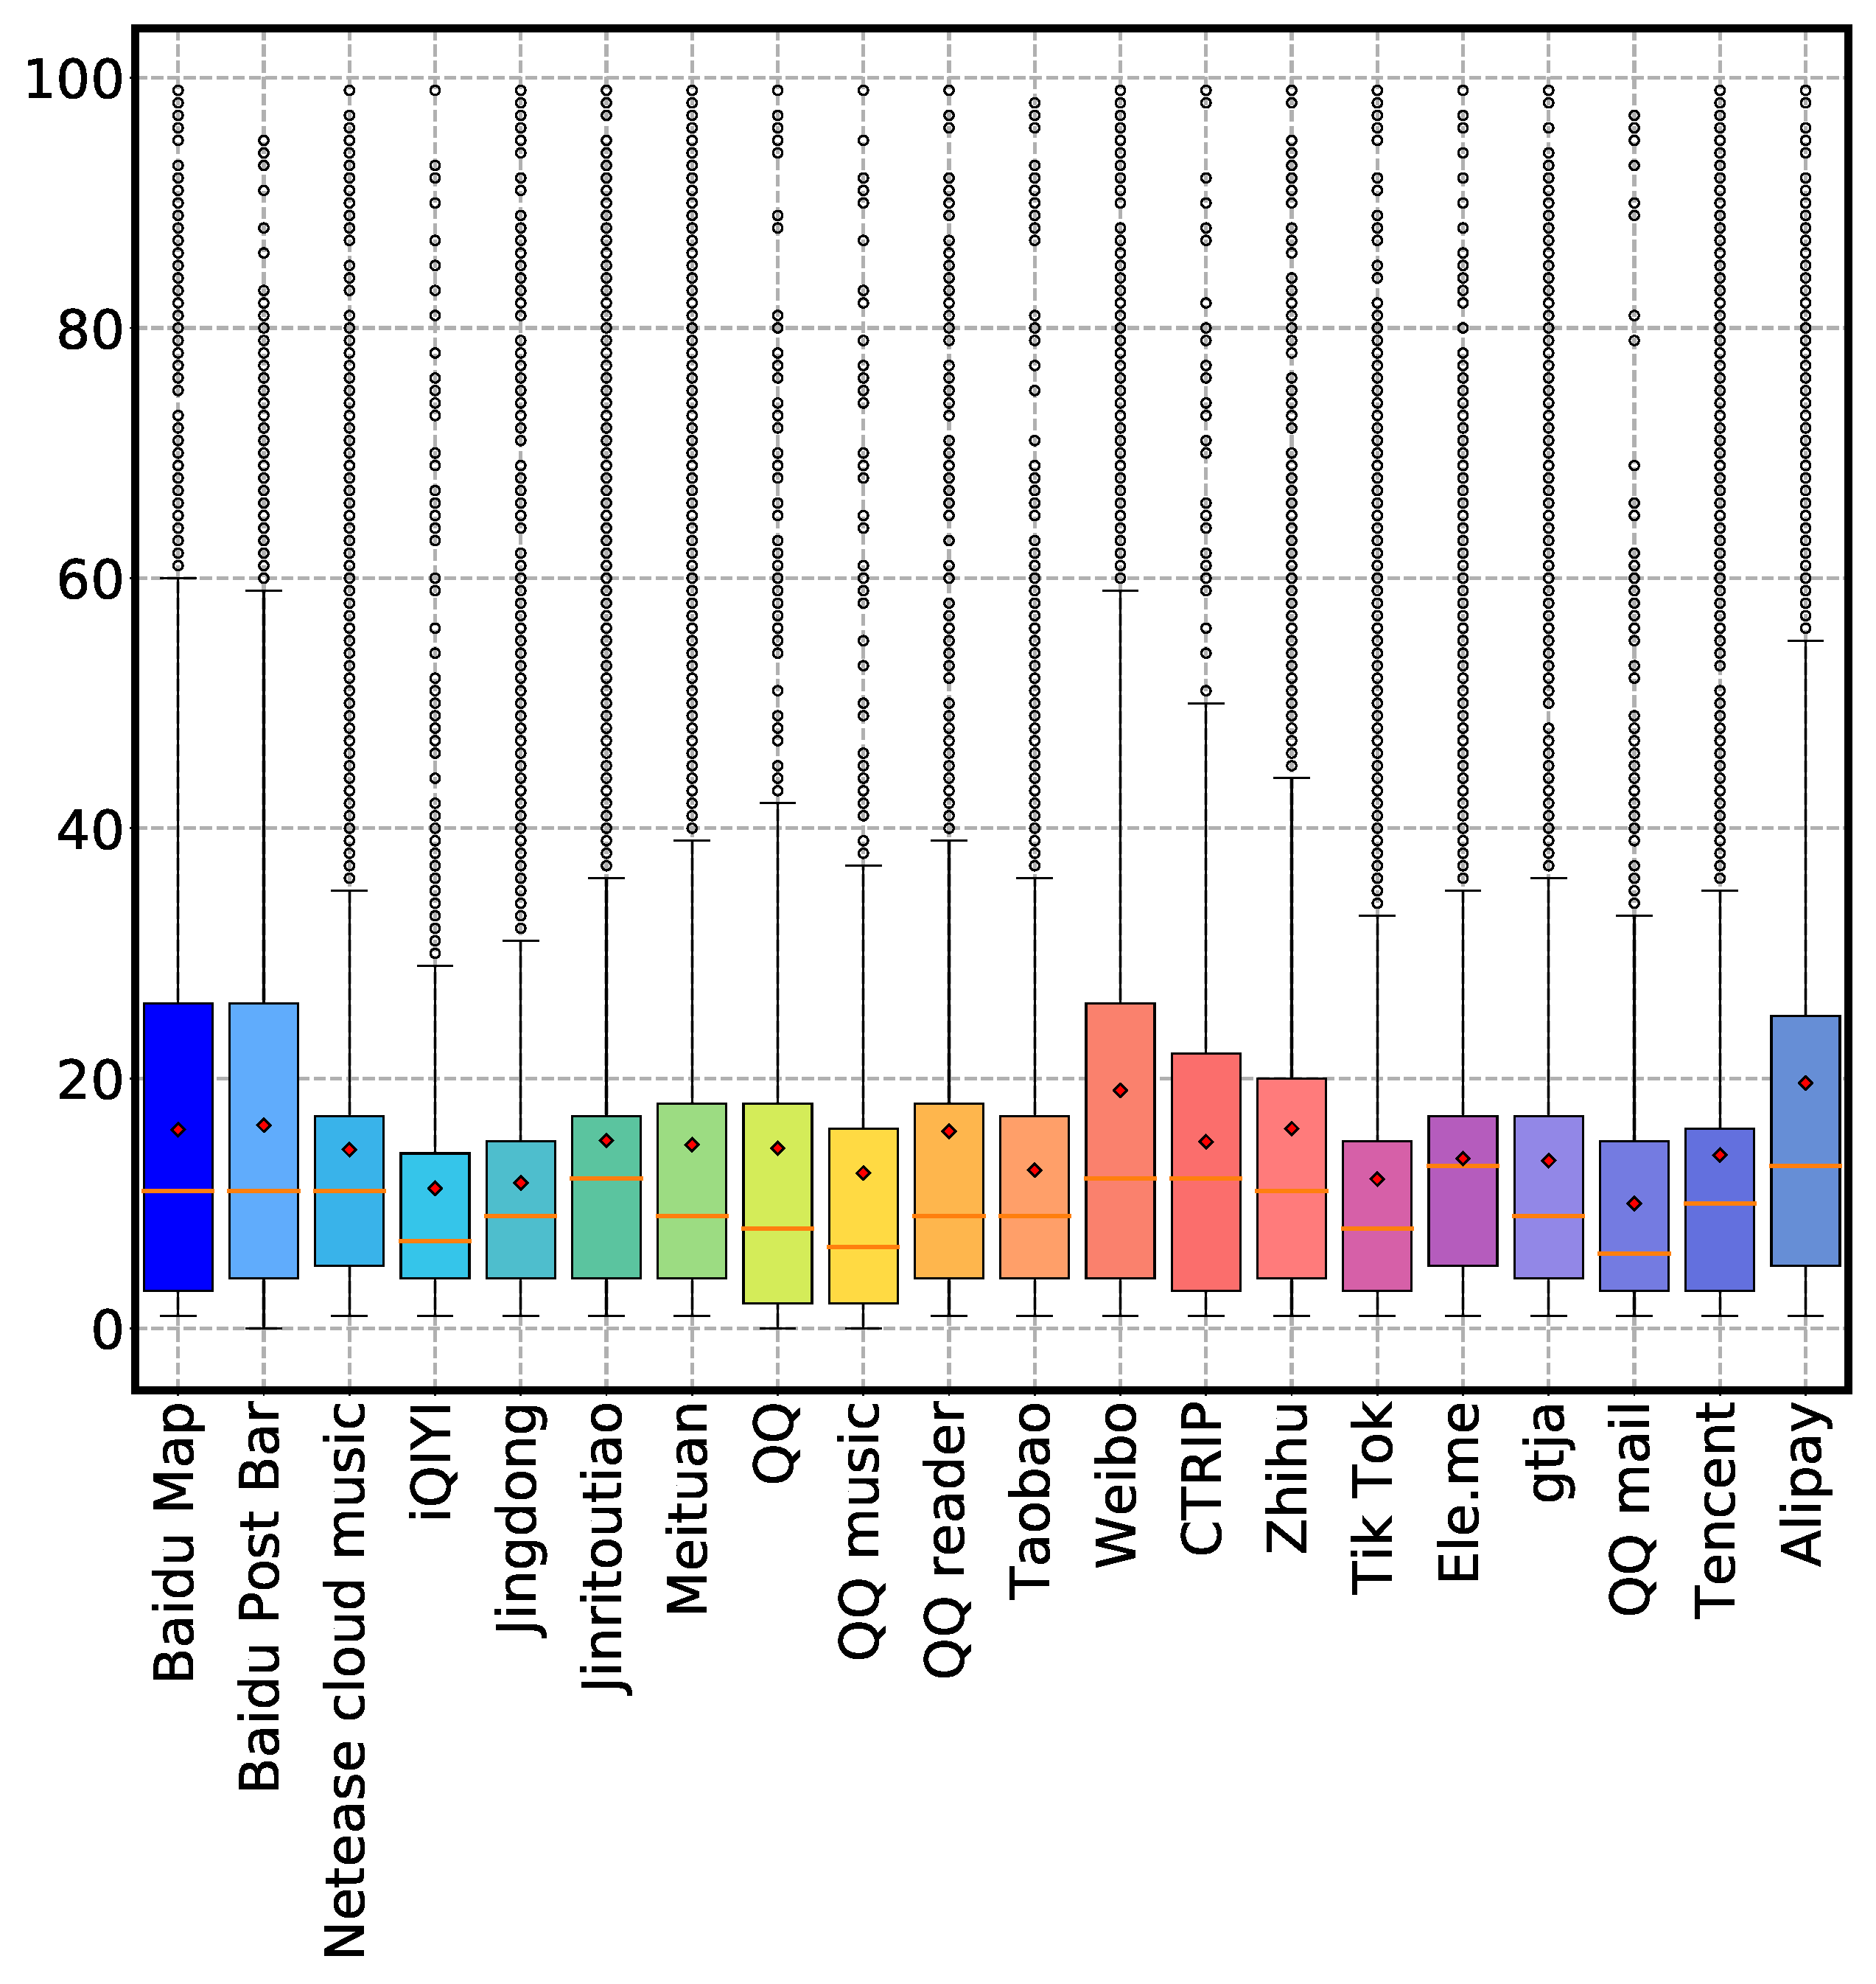
\includegraphics[width=0.80\textwidth]{packet-size-eda.eps}
	\bicaption{数据包大小分布。}{Packet size distribution.}
	\label{fig:packet-size-eda}
\end{figure}


\subsubsection{视图特征矢量化}
确立识别视图后,将三种视图转换为矢量表示。

\emph{(i)}对于数据包大小视图,通过计算前M个数据包的大小(用-1填充),形成了$ M $维矢量$ v_ {ps} $。

\emph{(ii)}对于内容类型视图,通过将值内容类型字段扩展为前M个数据包(用-1填充)来形成$ M $维矢量$ v_ {ct} $,其范围从0到255 。

\emph{(iii)}对于负载视图,通过将有效载荷字节值视为相应的ASCII码,对于每一个数据包取前N个字节,形成一个$ M \times N $维向量$v_{pb}$,然后进一步转换为0-255( 用-1填充)。

以上涉及到的超参数M和N将在本章后面进行详细分析。


\subsection{多视图特征学习}
针对负载视图、内容类型视图和数据包大小视图分别采用一维卷积神将网络、循环神经网络和一维卷积神经网络提取抽象的特征。

\begin{itemize}
	\item \textbf{负载视图特征学习:} 
	%
	本章使用一维卷积神经网络处理 $v_{pb}$向量,如公式:\ref{eqn:1D-payload}。在处理过程中, 使用了两层卷积神经网络, 每一层卷积的卷积核数量是 64, 卷积核的大小是$1 \times 3$, 卷积操作中本章采用的是max pooling。经过处理后,原始的负载部分的转换为64维的向量 $\alpha$.
	%
	\begin{equation}
	\label{eqn:1D-payload}
		\alpha = \mathit{1\!D\!-\!C\!N\!N}(v_{pb})
	\end{equation}
	
	\item \textbf{内容类型视图特征学习:} 
	内容类型是一个用257维的one-hot编码的稀疏向量,每一个取值之间的距离为$\sqrt{2}$,one-hot编码方式不能够有效表示上下文关系,所以本章引入了Embedding操作将这个257维的稀疏表示映射为一个16维的实数向量,这种表示方法有效保留了上下文关系。Embedding层需要学习一个转换向量,其大小为 $ (vocab\_size, embedding\_dim) $,Embedding基本上是一个矩阵,可以认为是从离散且稀疏的ont-hot向量到连续且密集的潜在空间的转换。经过Embedding操作后,使用循环神经网络从内容类型视图序列特征中提取抽象特征,形式上如公式\ref{eqn:1D-content-type}所示。 
	\begin{equation}
	\label{eqn:1D-content-type}
		\gamma = \mathit{R\!N\!N}(Embedding(v_{ct}))
	\end{equation}
	
	经过RNN处理后,content type视图被转换为一个64维的向量$\gamma$
	
	\item \textbf{数据包大小视图特征学习:}
	如公式\ref{eqn:1D-packet-size}所示,$v_{ps}$向量和处理负载部分的一样,使用一维卷积神经网络进行处理, 所不同的是输入的向量大小为数据包的数目。
	
	经过一维卷积神经网络的处理后, 数据包大小序列被转换为一个64维的向量 $\beta$.
	%
	\begin{equation}
	\label{eqn:1D-packet-size}
		\beta = \mathit{1D\!-\!C\!N\!N}(v_{ps})
	\end{equation}
	%

\end{itemize}


\subsection{应用识别}
如公式\ref{eqn:feature-combine}所示,将三个不同的抽象特征连接在一起以形成192维向量,然后将其输入到完全连接的层。完全连接层的输出$ x $,将用作softmax回归的输入,以识别流量。
\begin{equation}
\label{eqn:feature-combine}
	\delta = \alpha \oplus \beta \oplus \gamma
\end{equation}
三种不同的抽象特征共同优化同一类别目标,共同计算多类交叉熵损失,并通过反向传播算法\citep{rumelhart1986learning}更新三个神经网络的参数。
%
从数学上讲,输出预测$ Y $是应用 $ a_j $的概率由公式\ref{eqn:softmax}确定。
\begin{equation}
\label{eqn:softmax}
p(Y=j|x,W,b)=\mathit{softmax_j}(\emph{\textbf{W}}x + \emph{\textbf{b}})
% =\frac{e^{w_i^TZ+b_i}}{\sum_je^{w_j^TZ+b_j}}
\end{equation}

其中$ W $是完全连接层和softmax层之间的权重矩阵,而$ b $是偏移量。

如公式:\ref{eqn:argmax}所示,模型的预测值$y_{pd} $为概率最大的类别。
%
\begin{equation}
\label{eqn:argmax}
y_{pd}=argmax(p(Y=j|x,W,b)),\forall j \in \{1,2,3,...,C\}
\end{equation} 
%
AIBMF模型使用交叉熵 \citep{Boer2005A} 作为损失函数。

本文中所提到的研究识别模型的细节如表\ref{tab:AIBMF-layer}所示(此表是当超参数M=16,N=64时的情况)。



\begin{table}[!htbp]
    \bicaption{AIBMF网络。}{AIBMF network.}
    \label{tab:AIBMF-layer}
    \centering
    \footnotesize% fontsize
    \setlength{\tabcolsep}{4pt}% column separation
    \renewcommand{\arraystretch}{1.2}%row space 
    \begin{tabular}{|c|c|c|c|}
        \hline
        \textbf{网络层(类型)} & \textbf{输出层} & \textbf{参数个数} & \textbf{上一层网络}\\
        \hline
        \hline
        packetPayload (InputLayer) & (None, 1024) & 0 & \\
        \hline
        packetSize (InputLayer) & (None, 16) & 0 & \\
        \hline
        batch\_normalization\_1 (BatchNor) & (None, 1024) & 4096 & packetPayload[0][0] \\
        \hline
        batch\_normalization\_2 (BatchNor) & (None, 16) & 64 & packetSize[0][0] \\     
        \hline
        reshape\_1 (Reshape) & (None, 1024, 1) & 0 & batch\_normalization\_1[0][0] \\
        \hline
        reshape\_2 (Reshape) & (None, 16, 1) & 0 & batch\_normalization\_2[0][0] \\
        \hline
        layer\_conv\_1 (Conv1D) & (None, 1022, 64) & 256 & reshape\_1[0][0] \\
        \hline
        layer\_conv\_3 (Conv1D) & (None, 14, 64) & 256 & reshape\_2[0][0] \\
        \hline
        max\_pooling1d\_1 (MaxPooling1D) &  (None, 1020, 64) & 0 & layer\_conv\_1[0][0] \\ 
        \hline
        max\_pooling1d\_3 (MaxPooling1D) & (None, 12, 64) & 0 & layer\_conv\_3[0][0] \\
        \hline
        layer\_conv\_2 (Conv1D) & (None, 1020, 32) & 6176 & max\_pooling1d\_1[0][0] \\  
        \hline
        recordTypes (InputLayer) & (None, 16) & 0 & \\     
        \hline
        layer\_conv\_4 (Conv1D) & (None, 12, 32) & 6176 & max\_pooling1d\_3[0][0] \\
        \hline
        max\_pooling1d\_2 (MaxPooling1D) & (None, 1018, 32) & 0 & layer\_conv\_2[0][0] \\
        \hline
        embedding\_1 (Embedding) & (None, 16, 32) & 8224 & recordTypes[0][0] \\
        \hline
        max\_pooling1d\_4 (MaxPooling1D) &  (None, 10, 32) & 0 & layer\_conv\_4[0][0] \\
        \hline
        flatten\_1 (Flatten) & (None, 32576) & 0 & max\_pooling1d\_2[0][0] \\
        \hline
        lstm\_1 (LSTM) & (None, 16) & 3136 & embedding\_1[0][0] \\
        \hline
        flatten\_2 (Flatten) & (None, 320) & 0 & max\_pooling1d\_4[0][0] \\ 
        \hline
        dense\_1 (Dense) & (None, 64) & 2084928 & flatten\_1[0][0] \\
        \hline
        dense\_2 (Dense) & (None, 64) & 1088 & lstm\_1[0][0] \\
        \hline
        dense\_3 (Dense) & (None, 64) & 20544 & flatten\_2[0][0] \\
        \hline
        concatenate\_1 (Concatenate) & (None, 192) & 0 & dense\_1[0][0],dense\_2[0][0],dense\_3[0][0] \\
        \hline
        main\_output (Dense) & (None, 20) & 3860 & concatenate\_1[0][0] \\
        \hline
        \hline
        \textbf{总共参数} & \multicolumn{3}{|c|}{2,138,804} \\
        \textbf{可训练的参数} & \multicolumn{3}{|c|}{2,136,724} \\
        \textbf{不可训练的参数} & \multicolumn{3}{|c|}{2,080} \\
        \hline
    \end{tabular}
\end{table}    


\section{实验评估}
\subsection{评估指标}
为了对AIBMF在HTTPS流量数据上的识别性能进行合理有效的定量评估,本文介绍了一些基本指标:真阳性(True Positive, TP),假阴性(False Negative, FN),真阴性(True Negnative, TN)和假阳性(False Positive, FP),如表~\ref{tab:confusion-matrix}所示,具体含义为:TP是指属于应用$i$的流最终没有被识别为应用$i$的流的数量;FN是指属于应用$i$的流最终没有被识别为应用$i$的流的数量;TN是指不是应用$i$的流最终没有被识别为应用$i$的流的数量;FP是指不属于应用$i$的流最终被识别为应用$i$的流的数量。

\begin{table}[!htbp]
    \bicaption{识别结果的混淆矩阵。}{Confusion matrix of classification results.}
    \label{tab:confusion-matrix}
    \centering
    \footnotesize% fontsize
    \setlength{\tabcolsep}{4pt}% column separation
    \renewcommand{\arraystretch}{1.2}%row space 
    \begin{tabular}{l|l|c|c|c}
        \multicolumn{2}{c}{}&\multicolumn{2}{c}{\textbf{预测结果}}&\\
        \cline{3-4}
        \multicolumn{2}{c|}{} & \textbf{正类} & \textbf{负类} & \multicolumn{1}{c}{\textbf{总计}}\\
        \cline{2-4}
        \multirow{2}{*}{\textbf{真实情况}} & \textbf{正类} & 真正类(TP) & 假负类(FN) & $TP+FN$\\
        \cline{2-4}
        & \textbf{负类} & 假正类(FP) & 真负类(TN) & $FP+TN$\\
        \cline{2-4}
        \multicolumn{1}{c}{} & \multicolumn{1}{c} {\textbf{总计}} & \multicolumn{1}{c}{$TP+FP$} & \multicolumn{    1}{c}{$FN+TN$} & \multicolumn{1}{c}{$TP+FN+FP+TN$}\\
    \end{tabular}
\end{table}

基于TP、FN、TN和FP四个基本指标,引入准确率、精度、召回率和$F_1$值四个指标,具体介绍如下:准确率(\emph{Accuracy, ACC})表示分类正确的样本占总样本的比率,由根据公式\ref{eqn:acc}计算;精度(\emph{Precision, P})表示预测为一个应用的流样本中确为该应用的流的比率,由根据公式\ref{eqn:P}计算;召回率(\emph{Recall, R})表示针对一个应用,预测正确的流量与属于该应用的所有流的比值,由公式\ref{eqn:R}计算;\emph{F1}值是结合精度和召回率两个指标的综合评价指标,由公式\ref{eqn:F1}计算。 

为了在所有$K$个应用上评估本文的方法,分别取$ P $,$ R $,$ F_1 $的平均值 --- 宏精度($ Macro \ Precision $),宏召回率($ Macro \ Recall $),宏$F_1$($ Macro \ F_1 $)作为整体指标,分别由公式\ref{eqn:macro-P},公式\ref{eqn:macro-R},公式\ref{eqn:macro-F1}计算而得。 

\begin{equation}
    \label{eqn:acc}
    ACC=\frac{TP+TN}{TP+TN+FP+FN}	
\end{equation}

\begin{subequations}
	\begin{equation}
	\label{eqn:P}
	P=\frac{TP}{TP+FP}
	\end{equation}
	
	\begin{equation}
	\label{eqn:macro-P}
	Macro\ Precision=\frac{1}{K}\sum_{i=1}^{K}P_i
	\end{equation}
	
\end{subequations}

% ===========
% EQUATION:08
% ===========
\begin{subequations}
	\begin{equation}
	\label{eqn:R}
	R=\frac{TP}{TP+FN}	
	\end{equation}
	
	\begin{equation}
	\label{eqn:macro-R}
	Macro\ Recall=\frac{1}{K}\sum_{i=1}^{K}R_i
	\end{equation}
\end{subequations}


\begin{subequations}
	\begin{equation}
	\label{eqn:F1}
	F_1=2\frac{P\times R}{P+R}
	\end{equation}
	
	\begin{equation}
	\label{eqn:macro-F1}
	Macro\ F_1=\frac{1}{K}\sum_{i=1}^{K}F_{1i}
	\end{equation}
\end{subequations}


\subsection{实验环境和数据集划分}
\subsubsection{实验环境}
本文所需的实验环境见表~\ref{tab:experiment-enviorment}。
\begin{table}[!htbp]
    \bicaption{实验所需的软硬件环境。}{Hardware and software environment of experiments.}
    \label{tab:experiment-enviorment}
    \centering
    \footnotesize% fontsize
    \setlength{\tabcolsep}{4pt}% column separation
    \renewcommand{\arraystretch}{1.2}%row space 
    \begin{tabular}{lcc}
        \hline
        \multirow{3}{*}{硬件} & CPU & 24 Intel (R) Xeon CPU E5-2650 v4 @ 2.2GHz \\
        & GPU & 2 GTX TITAN X \\
        & RAM & 128GB\\
        \hline
        \multirow{5}{*}{软件} & 操作系统 & Ubuntu 16.04 LTS\\
        & 编程语言 & Python 3.6, Linux bash \\
        & 深度学习框架 & Tensorflow 1.12,Keras 2.2.4\\
        & 机器学习框架 & scikit-learn 0.22.1\footnotemark[1]\\
        & 重要Python包 & Scapy\footnotemark[2], Pandas\footnotemark[3], Numpy\footnotemark[4], Matplotlib\footnotemark[5] \\
        \hline
    \end{tabular}

\end{table}
\footnotetext[1]{https://scikit-learn.org/}
\footnotetext[2]{https://scapy.net/}
\footnotetext[3]{https://pandas.pydata.org/}
\footnotetext[4]{https://numpy.org/}
\footnotetext[5]{https://matplotlib.org/}

\subsubsection{数据集划分}
本章针对所采集的前20个应用共计10,000多条样本进行训练和识别,将100,000多个带有标签的样本分为两个部分:训练集和测试集。为了确保随机性,对数据进行了随机操作,其中训练集占90%,测试集占10%。


\subsection{敏感性参数M的分析}
如第三章所述,敏感性参数M是指一条数据流样本中数据包的个数。为了分析参数M对于识别效果的影响,针对前20个应用100,000多个流数据,并研究了各种应用的数据包计数分布。如图\ref{fig:packet-count-all}所示,超过100,000个流的数据集中的单条流数据包计数超过16只占32%,针对每一条流,取用不同的数据包的数目进行对比实验,如图\ref{fig:packet-count-acc},发现,随着数据包的数目的增加,模型的识别效果也在持续增加,当数据包的数目增加为16个的时候,准确率达到93.8\%。之后随着数据包数量的增加,识别的效果不再由明显的变化,但是经过分析,随着数据包数目的增加,模型所需要的空间复杂度和时间复杂度都会增加。在这里,将数据包的数目取为16。

\begin{figure}[!htbp]
    \centering
    \begin{subfigure}[b]{0.45\textwidth}
      \includegraphics[width=\textwidth]{Packet-count-all.eps}
      \caption{}
      \label{fig:packet-count-all}
    \end{subfigure}%
    ~% add desired spacing
    \begin{subfigure}[b]{0.45\textwidth}
      \includegraphics[width=\textwidth]{Payload-size-acc.eps}
      \caption{}
      \label{fig:packet-count-acc}
    \end{subfigure}
    ~% add desired spacing

    \bicaption{超参数M。(a)流中数据包数统计 ,(b) 不同数据包数量识别效果。}{Parameter M.(a)Statistics in  Packet Count, (b)Performance of Different M .}
    \label{fig:oaspl}
\end{figure}


\subsection{敏感性参数N的分析}
如第三章所述,敏感性参数N是指流样本中单个数据包所截取的字节数。为了分析参数N对于识别效果的影响,进行了一系列比较实验。如图\ref{fig:payload-size}所示,每个数据包以不同的长度截取,随着截取长度的增加,1D-CNN的识别能力增强。当采用前64个字节时,测试集的准确性为93.34\%。在64个字节的长度之后,精度会非常缓慢地增加,并且增益随着字节数的增加而降低且神经网络的时间复杂度和空间复杂度将显着增加,因此每个数据包的长度设置为64。

\begin{figure}[!htbp]
	\centering
	\includegraphics[width=0.45\textwidth]{Packet-count-acc.eps}
	\bicaption{超参数N。}{Parameter N.}
	\label{fig:payload-size}
\end{figure}

\subsection{不同深度学习模型方法对比}
在实验的过程中,如图\ref{fig:performance-dl},分别比较了仅仅使用一维卷积神经网络、二维卷积神经网络处理负载视图和AIBMF模型训练的过程,对比了在识别的过程中,损失和准确率的变化过程。发现在训练的过程中,AIBMF模型损失下降更快,即更快收敛,准确率也领先于仅使用一维卷积神经网络和仅使用二维卷积神经网络的方法。
\begin{figure}[!htbp]
    \centering
    \begin{subfigure}[b]{0.45\textwidth}
      \includegraphics[width=\textwidth]{AIBMF-training-loss.png}
      \caption{}
      \label{fig:acc-training}
    \end{subfigure}%
    ~% add desired spacing
    \begin{subfigure}[b]{0.45\textwidth}
      \includegraphics[width=\textwidth]{AIBMF-training-acc.png}
      \caption{}
      \label{fig:loss-training}
    \end{subfigure}
    ~% add desired spacing

    \bicaption{不同深度学习模型表现。(a) 准确率变化,(b) 损失变化。}{Performance of Different DL model (a) Accuracy over Training, (b) Loss over Training.}
    \label{fig:performance-dl}
\end{figure}



\subsection{基于流统计特征的方法}
本文的研究工作还对比了机器学习的方法,首先使用特征工程的方法构建了23种特征,见表\ref{tab:statistical-feature},其中7种特征是HTTPS协议相关的,其余的16种特征是流量分析工作常用的特征,属于协议无关的特征。

\begin{longtable}{ccc}
    \bicaption{统计特征。}{Statistical Feature.}\\
    \label{tab:statistical-feature}\\
	\hline
	\textbf{统计特征} & \textbf{含义} & \textbf{是否协议相关?} \\
	\hline
	\endfirsthead
	\multicolumn{3}{c}%
        {\bfseries\small \tablename\ \thetable\ {续表。}}\\
	\hline
	\textbf{统计特征} & \textbf{含义} & \textbf{是否协议相关?} \\
	\hline
	\endhead
	\hline \multicolumn{3}{r}{\textit{续表见下页}}\\
	\endfoot
	\hline
	\endlastfoot
	Packet counts & 数据包个数& 否\\
	TTL max & TTL最大值 & 否\\
	TTL min & TTL最小值 & 否\\
	TTL mean & TTL平均值 & 否\\
	TTL median & TTL中位数 & 否\\
	TTL var & TTL方差 & 否\\
	packet\_length max & 数据包长度最大值 & 否\\
	packet\_length min & 数据包长度最小值 & 否\\
	packet\_length mean & 数据包长度平均值 & 否\\
	packet\_length median & 数据包长度中位数 & 否\\
	packet\_length var & 数据包长度方差 & 否\\
	window max & 窗口最大值 & 否\\
	window min & 窗口最小值 & 否\\
	window mean & 窗口平均值 & 否\\
	window median & 窗口中位数 & 否\\
	window var & 窗口方差 & 否\\
	session\_id\_length max & session id长度 & 否\\
	client\_extensions\_length max & client extensions长度最大值 & 是\\
	client\_extensions\_length min & client extensions长度最小值 & 是\\
	client\_extensions\_length mean & client extensions长度平均值 & 是\\
	client\_extensions\_length median & client extensions长度中位数 & 是\\
	client\_extensions\_length var & client extensions长度方差 & 是\\
	client\_ciphers counts & 客户端加密组件种类 & 是\\
	server\_cipher & 服务端加密组建类型 & 是\\
	\hline
\end{longtable}
针对提取的23种特征,分别使用了随机森林,支持向量机和单层神经网络进行训练和识别。如表\ref{tab:ml-performance}所示,和本章提出的AIBMF模型相比较,基于机器学习的方法在识别能力弱,AIBMF模型在三个参数上均领先于其他的识别模型。

\begin{table}[!htbp]
    \bicaption{机器学习和AIBMF识别效果对比。}{Comparation the Performance between ML and AIBMF.}
    \label{tab:ml-performance}
    \centering
    \footnotesize% fontsize
    \setlength{\tabcolsep}{4pt}% column separation
    \renewcommand{\arraystretch}{1.2}%row space 
	\begin{tabular}{ c  c  c  c }
		\hline
		\textbf{机器学习算法} & \textbf{宏精度} & \textbf{宏召回率} & \textbf{宏F1} \\
		\hline
		随机森林 & 0.8805 & 0.8172 & 0.8407 \\
		支持向量机 & 0.9214 & 0.5754 & 0.6676 \\
		DNN & 0.7362 & 0.6293 & 0.6562 \\
		\textbf{AIBMF} & \textbf{0.918} & \textbf{0.909} & \textbf{0.913} \\
		\hline
	\end{tabular}
\end{table}


\subsection{AIBMF模型识别效果}
如图\ref{fig:Performance-AIBMF-Baseline}所示,在本章使用的前20个应用的数据集上将AIBMF与\citet{Wang2017End}的工作进行了比较。 评估结果表明,AIBMF在精度,召回率和F1得分方面至少优于2.0%。
\begin{figure}[!htbp]
	\centering
	\includegraphics[width=0.45\textwidth]{Performance-AIBMF-Baseline.eps}
	\bicaption{AIBMF模型和Baseline的比较。}{AIBMF vs. Baseline.}
	\label{fig:Performance-AIBMF-Baseline}
\end{figure}


如图\ref{fig:AIBMF-confusematrix},针对20个移动应用1万条测试样本,绘制混淆矩阵来观察识别的效果。整体上,识别的效果非常好,其中大多数的错误是由于不同的应用之间可能共享服务所致,尤其针对那些由同一个公司开发的应用而言,识别能力存在一定的混淆。有一些应用将其API提供给了其他的应用作为公共接口,如百度地图,这给AIBMF模型的识别能力带来了一定的影响。另外在实验中,QQ软件的识别效果最差,主要原因是QQ使用的通信协议主要是UDP,第三章捕获的流量主要从Qzone捕获,该流量混合了许多其他应用的流量。





\begin{figure}[!htbp]
	\centering
	\includegraphics[width=0.6\textwidth]{AIBMF-confusematrix.png}
	\bicaption{AIBMF识别混淆矩阵。}{AIBMF classification confusematrix.}
	\label{fig:AIBMF-confusematrix}
\end{figure}


\section{本章小结}
人工定义的统计特征越复杂,流量识别任务的通用性就越差。但是,仅使用深度学习忽略协议设计的信息来处理有效负载,识别能力也受到限制。实际上,协议定义的一些有意义的信息(例如内容类型)提取代价很低,在流量分析中却很有用。因此,从多个角度分析HTTPS流量并组合不同的功能可能是将来加密流量分析中的有力选择。本章节提出了一种通过HTTPS流量进行应用识别的方法---AIBMF。该方法能够分析HTTPS应用流量并将HTTPS流量与特定的移动应用相关联。